\chapter{Présentation et Étude}


\section{Introduction}

Dans ce chapitre, nous entamons une plongée profonde dans notre projet de conversion de wireframes dessinées à la main en interfaces web fonctionnelles. Nous examinerons les enjeux, les défis et les objectifs qui sous-tendent ce projet ambitieux. Nous explorerons également les méthodologies de travail que nous avons choisies pour garantir le succès de notre entreprise.

\section{Présentation générale du projet}

\subsection{Problématique}

Le développement d'une interface web implique une compréhension précise des besoins des clients. Cependant, la communication entre les clients non techniques et les développeurs peut être entravée par des barrières telles que des langages techniques complexes ou des difficultés à exprimer des idées visuelles de manière précise. Notre projet vise à surmonter ces obstacles en proposant une solution innovante de conversion automatique de wireframes en code HTML/CSS.

\subsection{Travail demandé}

Nous nous engageons à développer une application intuitive qui permettra aux utilisateurs de télécharger des wireframes dessinées à la main et de les convertir en interfaces web interactives en quelques clics. Pour atteindre cet objectif, nous devrons non seulement développer un algorithme de reconnaissance d'image avancé, mais aussi concevoir une interface utilisateur conviviale et esthétique.

\subsection{Méthodologie adoptée}

Nous avons opté pour une approche agile basée sur la méthodologie SCRUM pour la gestion de notre projet. SCRUM favorise la collaboration, la flexibilité et la livraison continue de fonctionnalités à valeur ajoutée. Cette approche itérative nous permettra de répondre rapidement aux changements de besoins des utilisateurs et d'itérer sur notre produit de manière efficace.

\subsubsection{Choix de la Méthodologie}

SCRUM a été choisi pour sa capacité à offrir une structure flexible et adaptable à notre équipe de développement. En favorisant la communication et la transparence, SCRUM nous permettra de rester alignés sur les objectifs du projet tout en nous adaptant aux défis rencontrés en cours de route.

\subsubsection{Présentation de SCRUM}

SCRUM est une méthodologie de développement agile qui repose sur des cycles de développement courts appelés "sprints". Chaque sprint, généralement d'une durée de deux à quatre semaines, se concentre sur la livraison d'un ensemble défini de fonctionnalités. Les équipes SCRUM se réunissent régulièrement pour planifier, collaborer et évaluer leur travail, ce qui favorise la transparence et l'efficacité.

\section{Étude préalable}
\subsection{Étude de l'Existant}
\subsection{Étude préalable}

\subsubsection{Uizard.io}
\begin{figure}[h]
    \centering
    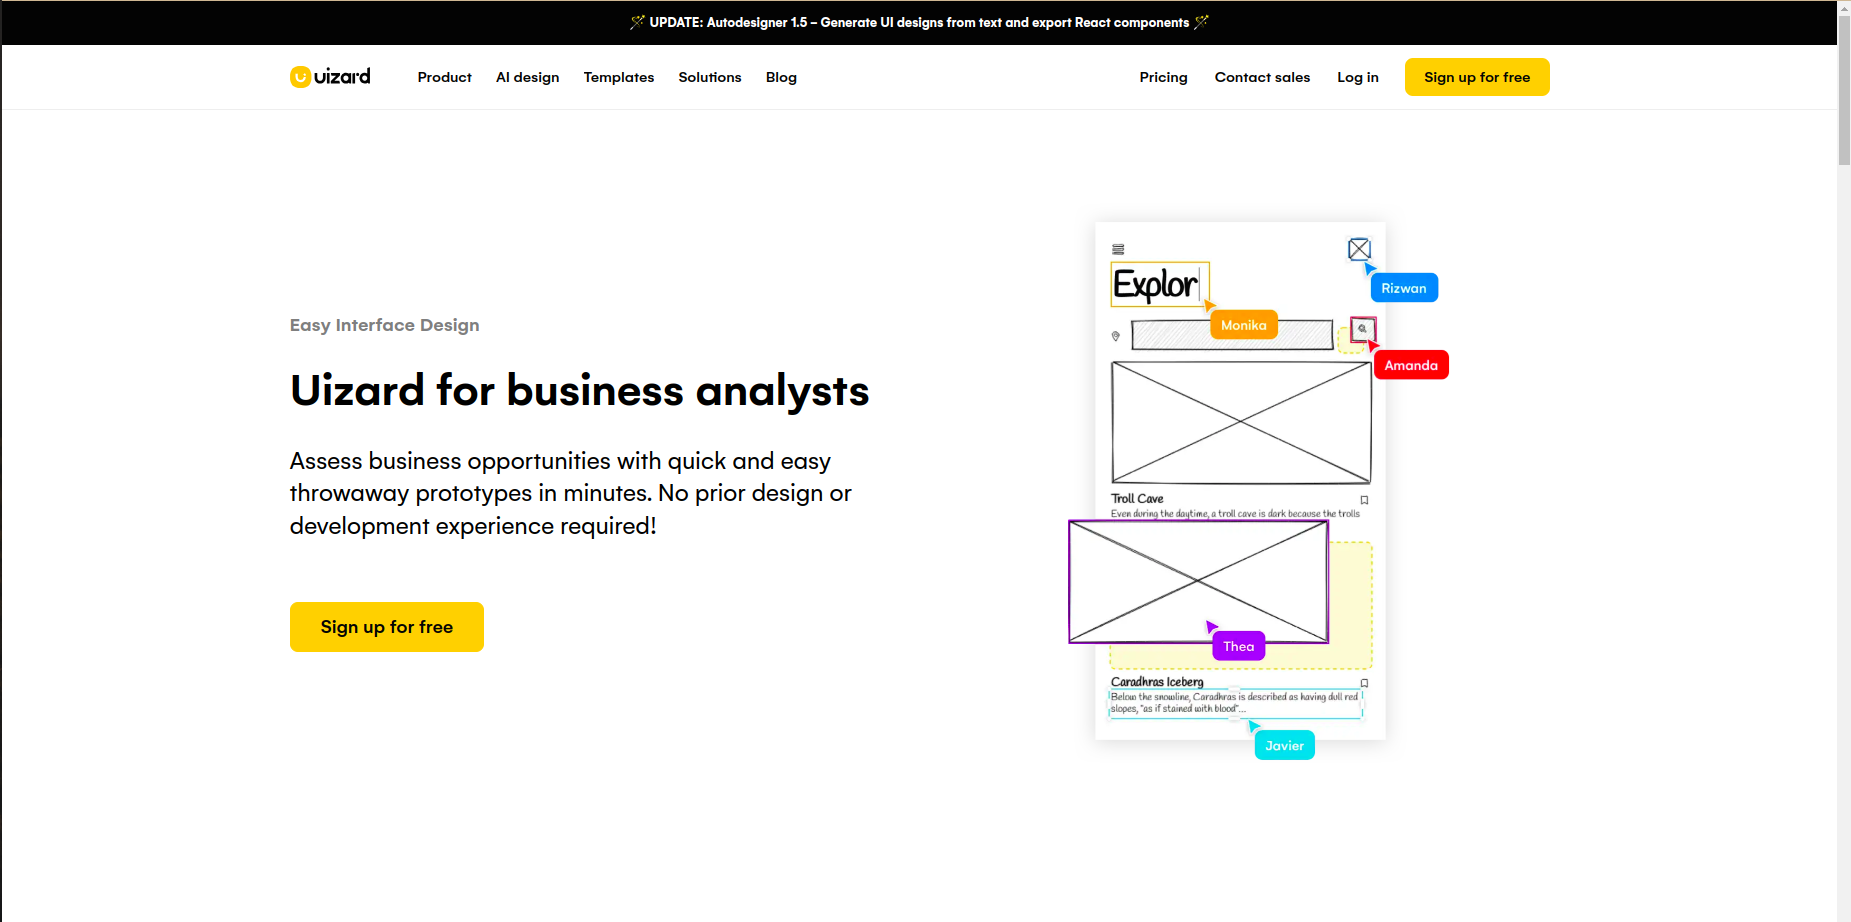
\includegraphics[width=0.45\textwidth]{Capture d’écran du 2024-02-07 15-40-13.png}
    \caption{Interface utilisateur de Uizard.io}
    \label{fig:uizard_interface}
\end{figure}
Uizard.io est une plateforme innovante qui offre une solution automatisée pour convertir les wireframes en code. Elle se distingue par sa rapidité de conversion et son interface intuitive, rendant le processus de développement web plus efficace et accessible pour les utilisateurs de tous niveaux.

\textbf{Avantages :}
\begin{itemize}
    \item \textbf{Automatisation efficace :} Uizard.io utilise des algorithmes avancés pour automatiser la conversion des wireframes en code. Cette automatisation permet de gagner du temps et d'optimiser le processus de développement, en transformant rapidement les idées de design en code fonctionnel.

    \item \textbf{Facilité d'Utilisation :} L'interface de Uizard.io est conçue pour être conviviale et intuitive. Elle offre une expérience utilisateur agréable, facilitant ainsi la création et la modification de wireframes, même pour les utilisateurs sans expérience en développement.
\end{itemize}

\textbf{Inconvénients :}
\begin{itemize}
    \item \textbf{Limitations avec des designs complexes :} Bien que Uizard.io soit efficace pour les wireframes simples et les designs standards, elle peut rencontrer des difficultés avec des designs complexes ou personnalisés. Dans ces cas, des ajustements manuels ou des interventions supplémentaires peuvent être nécessaires pour obtenir un code optimal.

    \item \textbf{Dépendance à l'IA :} La précision de la conversion de Uizard.io est étroitement liée à ses capacités d'intelligence artificielle. Cela signifie que la qualité du code généré peut varier en fonction des performances et des mises à jour de l'IA. Les utilisateurs doivent être conscients de cette dépendance et prêts à effectuer des vérifications et des ajustements si nécessaire.
\end{itemize}


\subsubsection{Sketch2Code}
\begin{figure}[h]
    \centering
    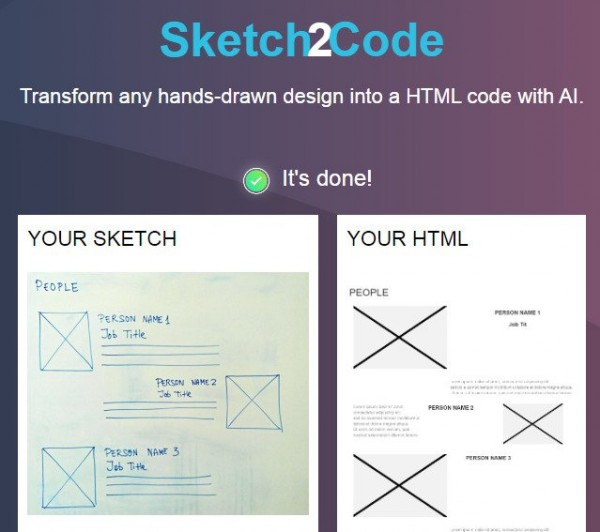
\includegraphics[width=0.45\textwidth]{convert image to html code.jpg}
    \caption{Interface utilisateur de Sketch2Code}
    \label{fig:sketch2code_interface}
\end{figure}
Sketch2Code se distingue par sa précision remarquable dans la conversion des wireframes en code et sa grande flexibilité qui permet d'adapter facilement les designs et les interactions. Cette plateforme offre une solution efficace pour les développeurs et les designers cherchant à transformer leurs idées de wireframes en réalité fonctionnelle.

\textbf{Avantages :}
\begin{itemize}
    \item \textbf{Précision dans la conversion :} Sketch2Code utilise des algorithmes avancés et des techniques d'analyse d'image pour assurer une conversion fidèle des wireframes en code. Cela garantit que le résultat final reflète exactement le design initial, minimisant ainsi les erreurs et les ajustements manuels.

    \item \textbf{Flexibilité pour les designs :} La plateforme offre une grande flexibilité pour gérer une variété de designs et d'interactions. Elle prend en charge différents éléments de design, tels que les boutons, les formulaires, les images et les icônes, et permet d'ajuster facilement les styles, les couleurs et les mises en page selon les besoins du projet.
\end{itemize}

\textbf{Inconvénients :}
\begin{itemize}
    \item \textbf{Connaissance en développement nécessaire :} Bien que Sketch2Code soit puissant, il nécessite une certaine connaissance en développement pour utiliser efficacement toutes ses fonctionnalités. Les utilisateurs doivent avoir une compréhension de base du HTML, du CSS et éventuellement du JavaScript pour optimiser le code généré et effectuer des ajustements personnalisés.

    \item \textbf{Limité en formats de fichier :} La plateforme peut être limitée en termes de formats de fichier supportés pour les wireframes. Elle pourrait ne pas prendre en charge certains formats populaires ou nécessiter des étapes supplémentaires pour convertir les fichiers dans un format compatible avec Sketch2Code.
\end{itemize}

\subsubsection{Adobe XD}
\begin{figure}[h]
    \centering
    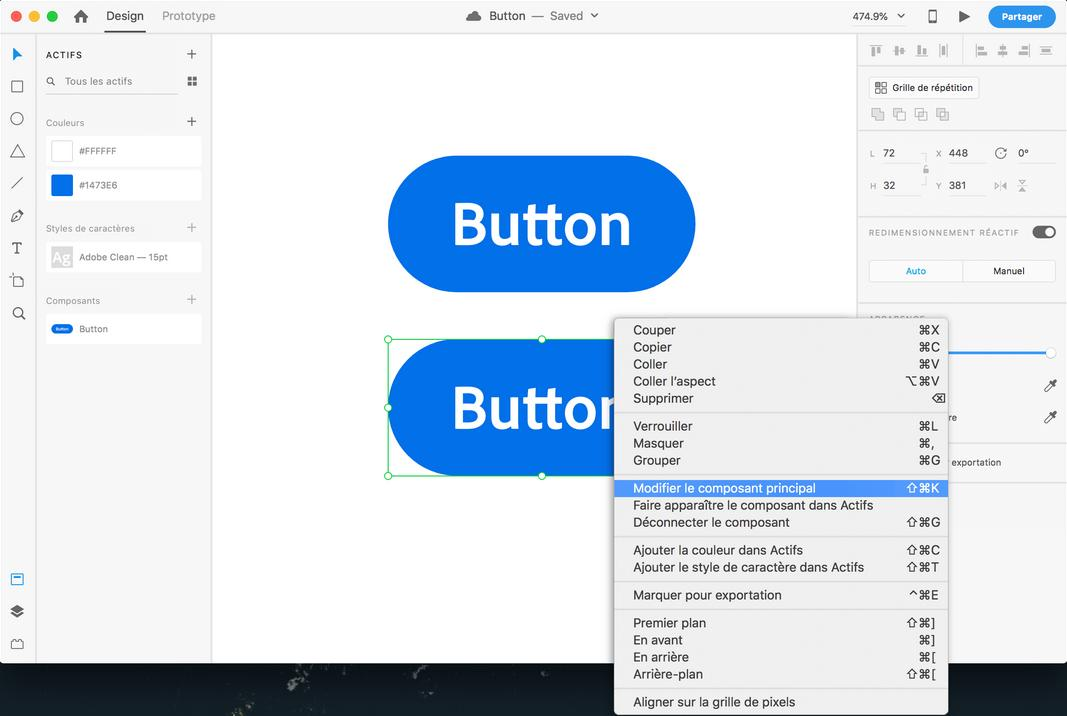
\includegraphics[width=0.45\textwidth]{-CFE4dK.jpg}
    \caption{Interface utilisateur de Adobe XD}
    \label{fig:adobe_xd_interface}
\end{figure}
Adobe XD est une solution de conception d'interfaces riche en fonctionnalités qui offre une intégration fluide avec d'autres produits Adobe. Elle est conçue pour les designers professionnels cherchant à créer des prototypes interactifs et des designs d'interface de haute qualité.

\textbf{Avantages :}
\begin{itemize}
    \item \textbf{Intégration avec Adobe :} Adobe XD s'intègre parfaitement avec d'autres produits Adobe, tels que Photoshop et Illustrator. Cette intégration permet aux designers de travailler de manière plus collaborative et efficace, en partageant facilement des éléments de design et des ressources entre différentes applications.

    \item \textbf{Fonctionnalités avancées :} Adobe XD offre une gamme complète de fonctionnalités avancées pour la conception d'interfaces, y compris des outils de prototypage interactif, des grilles et des guides de mise en page, ainsi que des fonctionnalités de collaboration en temps réel. Ces fonctionnalités permettent aux designers de créer des designs complexes et détaillés avec précision.
\end{itemize}

\textbf{Inconvénients :}
\begin{itemize}
    \item \textbf{Moins axé sur la conversion automatique :} Contrairement à d'autres plateformes spécialisées dans la conversion automatique des wireframes en code, Adobe XD est davantage axé sur la conception et le prototypage. Bien qu'il offre des outils pour faciliter le processus de développement, il peut nécessiter des étapes supplémentaires ou des plugins pour convertir efficacement les designs en code.

    \item \textbf{Nécessite Adobe Creative Cloud :} Pour accéder à Adobe XD et profiter de ses fonctionnalités complètes, les utilisateurs doivent s'abonner à Adobe Creative Cloud. Cela peut représenter un coût supplémentaire pour certains utilisateurs et nécessite une connexion internet pour l'installation et la mise à jour du logiciel.
\end{itemize}


\subsection{Solution proposée}

Notre solution innovante vise à développer une application personnalisée qui se démarque par sa capacité à convertir les wireframes en code de manière précise et efficace. En combinant des techniques avancées de reconnaissance d'image et des algorithmes optimisés, nous nous engageons à fournir une solution fiable et performante pour nos utilisateurs.

\textbf{Caractéristiques clés de notre solution :}
\begin{itemize}
    \item \textbf{Interface utilisateur intuitive :} Nous mettons l'accent sur la convivialité de notre interface utilisateur, en offrant une expérience utilisateur intuitive qui facilite la création et la modification de wireframes. L'interface sera conçue pour être accessible aux utilisateurs de tous niveaux, qu'ils soient débutants ou experts en conception d'interfaces.

    \item \textbf{Reconnaissance d'image avancée :} Notre solution intègrera un algorithme de reconnaissance d'image avancé qui permettra de détecter et d'analyser les wireframes téléchargés ou créés par les utilisateurs. Cet algorithme sera optimisé pour reconnaître les éléments de design, les interactions et les structures de page, garantissant ainsi une conversion précise en code.

    \item \textbf{Flexibilité et personnalisation :} Nous offrirons à nos utilisateurs la possibilité de personnaliser les designs et les interactions avant la conversion en code. Cette flexibilité permettra aux utilisateurs d'adapter les wireframes selon leurs besoins spécifiques et de créer des designs uniques et personnalisés.

    \item \textbf{Documentation complète :} Pour faciliter l'utilisation de notre application, nous fournirons une documentation complète et des guides d'utilisation détaillés. Cette documentation aidera les utilisateurs à comprendre les fonctionnalités de l'application, à suivre les étapes de conversion et à résoudre d'éventuels problèmes rencontrés.
\end{itemize}

En développant cette solution, notre objectif est de répondre aux besoins spécifiques de nos utilisateurs en offrant une plateforme robuste, flexible et facile à utiliser pour la conversion des wireframes en code. Nous sommes déterminés à fournir un outil qui facilite le processus de développement web et qui contribue à accélérer la mise sur le marché des projets de nos utilisateurs.

\section{Conclusion}

Ce chapitre a posé les bases de notre projet en présentant les défis et les enjeux associés à la conversion de wireframes dessinées à la main en interfaces web. Nous avons également défini notre méthodologie de travail, étudié les solutions existantes sur le marché et présenté notre solution proposée. Ce chapitre jette les fondations de notre projet et nous prépare à entamer le développement de notre application avec confiance et détermination.

